% Generated by scripts/build_slides.py from saved results.
\documentclass[aspectratio=169,11pt]{beamer}
\usepackage[T1]{fontenc}
\usepackage{lmodern}
\usepackage{graphicx}
\usepackage{booktabs}
\usepackage{amssymb}
\definecolor{banner}{HTML}{1B3A6B}
\definecolor{accent}{HTML}{2E6DB4}
\setbeamercolor{frametitle}{bg=banner,fg=white}
\setbeamercolor{title}{fg=banner}
\setbeamercolor{structure}{fg=banner}
\setbeamercolor{item}{fg=accent}
\setbeamertemplate{navigation symbols}{}
\setbeamertemplate{footline}[frame number]
\newcommand{\slide}[1]{\begin{frame}[plain]\makebox[\textwidth]{\includegraphics[width=\paperwidth]{figures/#1}}\end{frame}}

\title{When Trading Dries Up}
\subtitle{A liquidity signal for a long-only fund}
\author{Group 7 \\ Silver Fund}
\date{Built on 2011--2018}

\begin{document}
\begin{frame}\titlepage\end{frame}

\begin{frame}{The idea}
\begin{itemize}
\item A \textbf{liquidity event}: a stock suddenly trades far less than usual for it (measured against its own past year).
\item \textbf{Why it should matter:} most investors avoid illiquid stocks; only a small group of patient investors holds them, at a slightly lower price.
\item When a stock's trading collapses, it has to pass from its current holders to that small group.
  \begin{itemize}
  \item Sellers can only exit slowly, because volume has dried up; the few buyers need a lower price.
  \item So the price \textbf{walks down for months}. Shorting these stocks is costly, so nobody trades the drift away.
  \end{itemize}
\item We first remove anything the fund's six existing scores already capture.
\item Questions: is the effect real, and can our long-only fund make money from it?
\end{itemize}
\end{frame}

\begin{frame}{Bottom line}
\begin{itemize}
\item \textbf{Yes, it is real.} Stocks whose trading dries up keep falling: about 3\% behind similar stocks over the next year.
\item \textbf{Just avoiding them doesn't help:} +0.05\% to +0.10\% a year, not significant.
\item \textbf{Betting against them daily with the optimizer works:} long-only after trading costs +0.12\% a year (IR 1.04).
\item \textbf{It is small.} Use it as one input to the fund's alpha.
\end{itemize}
\end{frame}

\slide{matched_drift.png}
\slide{where.png}

\begin{frame}{It is not something we already know}
\centering
\small
\begin{tabular}{lr}
\toprule
 & How much less flagged stocks earn, \%/month ($t$) \\
\midrule
Had a liquidity event in the last month & 0.18 (2.5) \\
... also controlling for last month's return & 0.17 (2.4) \\
\bottomrule
\end{tabular}

\medskip
\raggedright\footnotesize Positive = flagged stocks earn less, which is what we bet on. Monthly regressions of next month's return, 2008--2018; every row also controls
for size, how illiquid the stock already was, its past-year return and its return two to three years ago, and the fund's six scores were removed before flagging.
Measured once a month, so it understates the first-weeks effect that daily trading captures.
\end{frame}

\begin{frame}{The simple idea doesn't work: just avoid these stocks}
\centering
\small
\resizebox{\linewidth}{!}{%
\begin{tabular}{lrrrrr}
\toprule
2011--2018 & Weight avoided & Return & Risk & IR ($t$) & IR, market removed \\
\midrule
Just avoid flagged stocks, daily & 8.6\% & +0.05\%/yr & 0.47\% & 0.11 (0.3) & $-$0.12 \\
Just avoid flagged stocks, monthly & 8.7\% & +0.10\%/yr & 0.43\% & 0.23 (0.7) & $-$0.12 \\
\midrule
Optimizer, daily, no shorting, costs & --- &+0.12\%/yr & 0.11\% & 1.04 (2.9) & --- \\
\bottomrule
\end{tabular}}

\medskip
\raggedright\footnotesize
\begin{itemize}
\item Hold the benchmark, sell every stock with a liquidity event in the last 63 days, give its weight to similar stocks.
\item It barely earns anything: these stocks are small, so dropping them tilts the portfolio in ways that add noise and swamp the effect.
\item The optimizer removes that noise and sizes each bet. That is what makes the signal pay.
\end{itemize}
\end{frame}

\begin{frame}{How we bet on it}
\textbf{Our alpha} (Grinold--Kahn form): \quad $\alpha_i = \sigma_i \times \bar d_{\,\text{age of event}}$
\begin{itemize}\small
\item $\sigma_i$: volatility; $\bar d$: how far flagged stocks fell behind similar stocks per unit of volatility (ages 1--21, 22--63 days), from earlier years. No recent event: $\alpha = 0$.
\end{itemize}
\medskip
\textbf{Optimizer:} \quad maximize $h^\top\alpha - \tfrac{\gamma}{2}\,h^\top V h - \lambda\cdot\text{spread costs}$, \ active risk $\le 1\%$
\begin{itemize}\small
\item $\gamma$ is fixed for a year: the previous year's median of the value that would put the no-limits portfolio at 1\% risk.
\item $\lambda$ (0.5--4) is picked each January from earlier years' net results.
\end{itemize}
\medskip

\centering\small
\resizebox{0.92\linewidth}{!}{\begin{tabular}{lccc}
\toprule
Constraint & No limits & Limited shorting + costs & No shorting + costs \\
\midrule
Fully invested: active weights sum to zero & $\checkmark$ & $\checkmark$ & $\checkmark$ \\
Zero beta to the benchmark & $\checkmark$ & $\checkmark$ & $\checkmark$ \\
Net zero within each size $\times$ liquidity group & $\checkmark$ & $\checkmark$ & $\checkmark$ \\
Short at most 0.25\% per stock ($b + h \ge -0.25\%$) & -- & $\checkmark$ & -- \\
Long-only: no weight below zero ($b + h \ge 0$) & -- & -- & $\checkmark$ \\
Pays half the bid--ask spread on every trade & -- & $\checkmark$ & $\checkmark$ \\
\bottomrule
\end{tabular}}

\medskip
\raggedright\scriptsize No limits pays no costs: it is the yardstick for the signal's full strength. No shorting stays small: the stocks it bets against hold little benchmark weight.
\end{frame}

\slide{vol_check.png}

\begin{frame}{Daily rebalancing, 2011--2018}
\begin{columns}[T]
\begin{column}{0.50\textwidth}
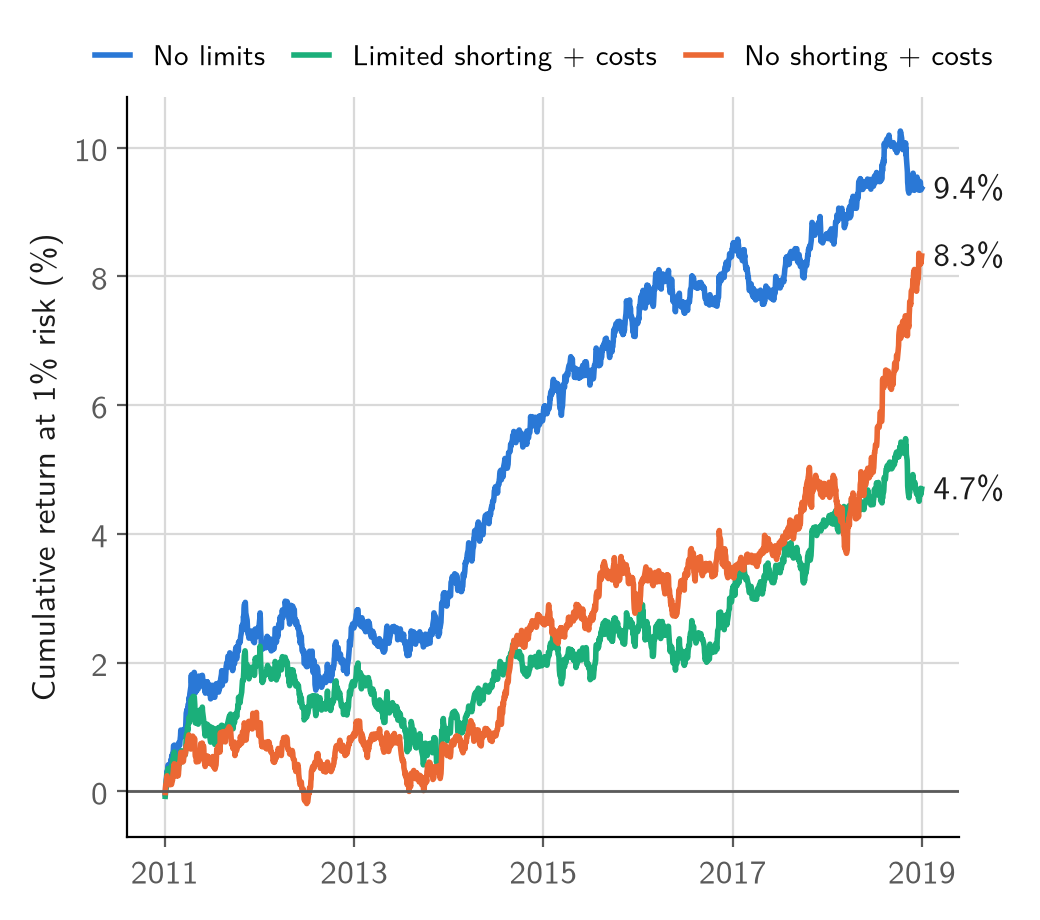
\includegraphics[width=\linewidth]{figures/pair_daily_fg.png}
\end{column}
\begin{column}{0.48\textwidth}
\vspace{10mm}
\scriptsize
\resizebox{\linewidth}{!}{%
\begin{tabular}{lrrr}
\toprule
 & No limits & Limited shorting + costs & No shorting + costs \\
\midrule
Active return, \%/yr & +1.30 & +0.57 & +0.12 \\
Active risk (realized) & 1.11\% & 0.97\% & 0.11\% \\
IR ($t$) & 1.17 (3.3) & 0.59 (1.7) & 1.04 (2.9) \\
Max drawdown & $-$1.53\% & $-$1.79\% & $-$0.16\% \\
Positive years & 8/8 & 6/8 & 7/8 \\
Turnover, $\times$/yr & 35.1 & 11.6 & 0.8 \\
TC vs no limits & ref. & 0.84 & 0.33 \\
Spread cost, \%/yr & 2.64 & 0.52 & 0.01 \\
\bottomrule
\end{tabular}}
\end{column}
\end{columns}
\vspace{1mm}
{\scriptsize Each period's line scaled to 1\% realized risk; the table shows actual numbers. No shorting = total weight $\ge 0$. Limited shorting = total weight $\ge -0.25\%$. + costs = pays half the spread on each trade; returns are after those costs. Fixed $\gamma$, risk $\le 1\%$.
TC = ex-ante transfer coefficient vs.\ no limits.\par}
\end{frame}

\begin{frame}{Monthly rebalancing, 2011--2018}
\begin{columns}[T]
\begin{column}{0.50\textwidth}
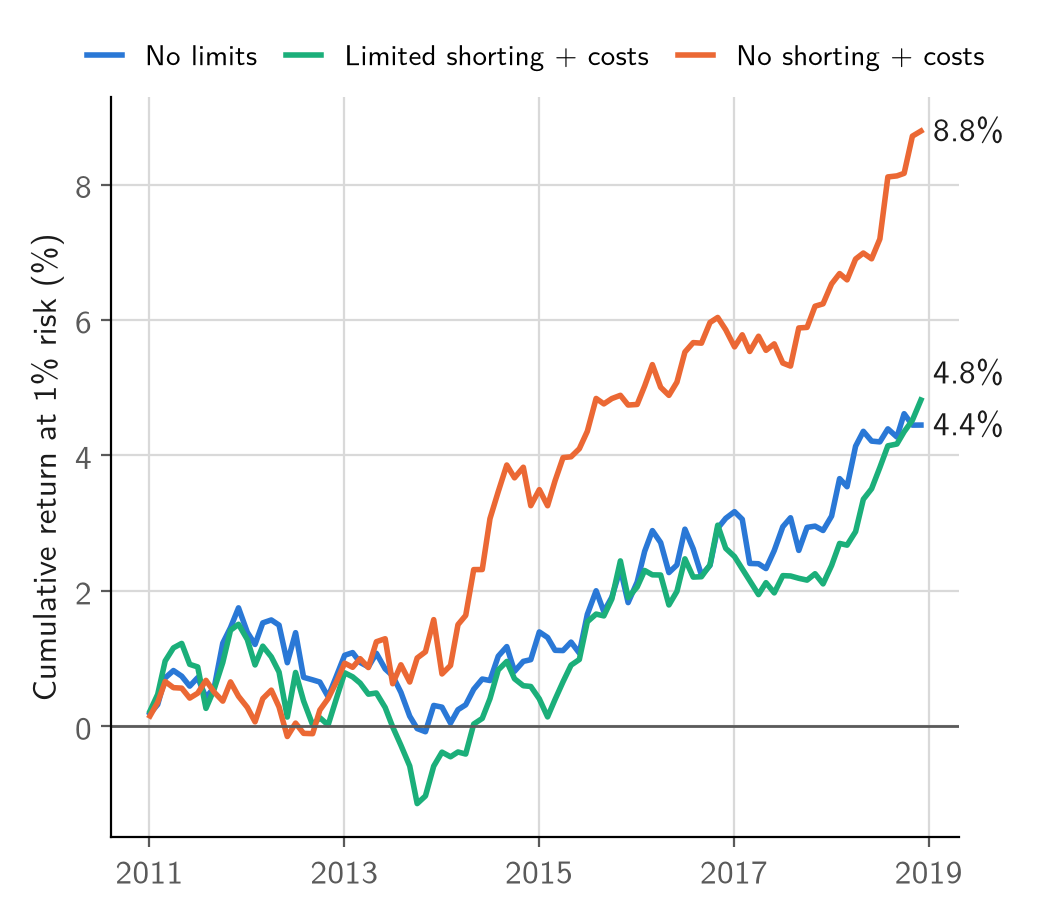
\includegraphics[width=\linewidth]{figures/pair_monthly_fg.png}
\end{column}
\begin{column}{0.48\textwidth}
\vspace{10mm}
\scriptsize
\resizebox{\linewidth}{!}{%
\begin{tabular}{lrrr}
\toprule
 & No limits & Limited shorting + costs & No shorting + costs \\
\midrule
Active return, \%/yr & +0.62 & +0.43 & +0.14 \\
Active risk (realized) & 1.11\% & 0.71\% & 0.12\% \\
IR ($t$) & 0.56 (1.6) & 0.60 (1.7) & 1.10 (3.1) \\
Max drawdown & $-$2.03\% & $-$1.89\% & $-$0.10\% \\
Positive years & 5/8 & 5/8 & 8/8 \\
Turnover, $\times$/yr & 11.3 & 2.9 & 0.3 \\
TC vs no limits & ref. & 0.58 & 0.24 \\
Spread cost, \%/yr & 1.04 & 0.13 & 0.01 \\
\bottomrule
\end{tabular}}
\end{column}
\end{columns}
\vspace{1mm}
{\scriptsize Each period's line scaled to 1\% realized risk; the table shows actual numbers. No shorting = total weight $\ge 0$. Limited shorting = total weight $\ge -0.25\%$. + costs = pays half the spread on each trade; returns are after those costs. Fixed $\gamma$, risk $\le 1\%$.
TC = ex-ante transfer coefficient vs.\ no limits.\par}
\end{frame}

\begin{frame}{How much to trust it}
\begin{itemize}
\item We built it on 2011--18 in four rounds; 2019--24 is held back for a final test.
\end{itemize}
\end{frame}

\begin{frame}{Conclusion}
\begin{itemize}
\item Stocks whose trading dries up keep falling for months: they must pass to a small group of patient buyers, and that hand-off is slow.
\item A long-only fund can make money from it, but only with the optimizer and daily trading.
\item It is small. Use it as one input to the fund's alpha, not on its own.
\item Next: combine it with the fund's scores and test the combined alpha, with trading costs.
\end{itemize}
\end{frame}

\begin{frame}[plain]\vfill\centering{\Large\textbf{\color{banner}Appendix}}\vfill\end{frame}

\slide{ic_by_year.png}

\begin{frame}{Appendix: what did we change, and when?}
\centering
\scriptsize
\begin{tabular}{lrr}
\toprule
Daily runs, \%/yr (IR), no costs & No limits & No shorting \\
\midrule
1. Flag that turns over daily & $-0.9$ ($-0.15$) & --- \\
2. Event clock & $-$2.77 ($-$0.49) & $-$0.12 ($-$0.24) \\
3. + no positive alpha, hedge with similar stocks & +3.23 (0.58) & +0.36 (1.48) \\
4. + alpha scaled by volatility & +6.84 (1.17) & +0.19 (1.82) \\
\bottomrule
\end{tabular}

\medskip
\raggedright\footnotesize
\begin{itemize}
\item Version 2: a flag that switched off after a few days missed most of the drift, so we gave each event an age.
\item Version 3: a noisy positive alpha for large stocks made the portfolio buy them; we stopped allowing positive alpha and hedged with similar stocks.
\item Version 4: calm stocks fell less than predicted (slide 9), so alpha now scales with volatility. Frozen before the 2019--24 test.
\end{itemize}
\end{frame}

\begin{frame}{Appendix: how we picked the short limit (2011--2018)}
\centering
\small
\begin{tabular}{lrrrr}
\toprule
Short limit per stock & Active risk (model) & IR & Turnover, $\times$/yr & Monthly IR \\
\midrule
0.05\% & 0.47\% & 1.14 & 15 & 0.74 \\
0.1\% & 0.85\% & 1.02 & 27 & 0.65 \\
\textbf{0.25\%} & \textbf{1.68\%} & \textbf{0.97} & \textbf{55} & \textbf{0.54} \\
0.5\% & 2.65\% & 0.94 & 90 & 0.54 \\
1\% & 3.90\% & 1.03 & 139 & 0.48 \\
2\% & 4.71\% & 1.12 & 175 & 0.50 \\
\bottomrule
\end{tabular}

\medskip
\raggedright\footnotesize Daily runs unless marked, earlier design (5\% risk target). The IRs are within noise of each other, so we chose the limit
by risk: 0.25\% (bold) sits between long-only and no limits. The same limit is used monthly.
\end{frame}

\begin{frame}{Appendix: every portfolio with and without trading costs (2011--2018)}
\centering
\scriptsize
\resizebox{\linewidth}{!}{%
\begin{tabular}{llrrrrr}
\toprule
 & & Return, \%/yr & IR ($t$) & Risk & Turnover, $\times$/yr & Spread cost, \%/yr \\
\midrule
\multicolumn{7}{l}{\textit{Daily rebalancing}} \\
No limits & no costs & +1.30 & 1.17 (3.3) & 1.11\% & 35 & 2.64* \\
No limits & with costs & +0.74 & 0.71 (2.0) & 1.05\% & 14 & 0.58 \\
Limited shorting (0.25\%) & no costs & +1.09 & 1.07 (3.0) & 1.02\% & 30 & 2.34* \\
Limited shorting (0.25\%) & with costs & +0.57 & 0.59 (1.7) & 0.97\% & 12 & 0.52 \\
No shorting & no costs & +0.16 & 1.97 (5.6) & 0.08\% & 2 & 0.08* \\
No shorting & with costs & +0.12 & 1.04 (2.9) & 0.11\% & 1 & 0.01 \\
\midrule
\multicolumn{7}{l}{\textit{Monthly rebalancing}} \\
No limits & no costs & +0.62 & 0.56 (1.6) & 1.11\% & 11 & 1.04* \\
No limits & with costs & +0.38 & 0.51 (1.4) & 0.76\% & 3 & 0.13 \\
Limited shorting (0.25\%) & no costs & +0.53 & 0.52 (1.5) & 1.02\% & 9 & 0.89* \\
Limited shorting (0.25\%) & with costs & +0.43 & 0.60 (1.7) & 0.71\% & 3 & 0.13 \\
No shorting & no costs & +0.07 & 0.98 (2.8) & 0.07\% & 1 & 0.02* \\
No shorting & with costs & +0.14 & 1.10 (3.1) & 0.12\% & 0 & 0.01 \\
\bottomrule
\end{tabular}}

\medskip
\raggedright\footnotesize Fixed $\gamma$, active risk $\le 1\%$. Costs = half the bid--ask spread on every trade, charged in the optimizer and in the returns;
* = what the portfolio would pay if traded alone (not charged). Risk = realized.
\end{frame}


\begin{frame}{Appendix: where does the return come from? (2011--2018)}
\centering
\small
\begin{tabular}{lrrr}
\toprule
Return, \%/yr & Event 1--21 days ago & Event 22--504 days ago & No recent event \\
\midrule
Daily, no limits & +14.88 & $-$3.43 & $-$4.64 \\
Daily, no shorting & +0.12 & +0.08 & $-$0.01 \\
Monthly, no limits & +8.02 & +0.09 & $-$4.09 \\
Monthly, no shorting & +0.09 & +0.06 & $-$0.05 \\
\bottomrule
\end{tabular}

\medskip
\raggedright\footnotesize Return earned on positions in stocks with a recent event, an older event, or none. In the no-limits runs the bets against flagged stocks are hedged
with similar stocks; small, illiquid stocks lag in general, so both sides show it and it cancels.
\end{frame}
\end{document}
